\documentclass[12pt,a4paper]{article}
\usepackage{fullpage}
\usepackage[margin=2cm]{geometry}
\usepackage{amsmath}
\usepackage{subfig}
\usepackage{graphicx}
\usepackage[justification=centering]{caption}
\begin{document}
\title{A comparison of two convolutional neural networks for landmarks detection }
\author{LE Van Linh and BEURTON-AIMAR Marie}
\date{October, 2017}
\maketitle
\begin{abstract}
	In this study, we presented a comparison between two convolution neural networks (CNNs) which are used to predict the landmarks on biological images. The first model was presented by Celia Cintas et al\cite{cintas2016automatic}. The model is used to predict the 45 landmarks on the human ear. The second model is proposed by us as a result of tutorial about Lassagne framework\cite{lasagne}. The proposed model is designed to predict 8 landmarks on beetle's pronotum. Both models have experimented on the dataset of pronotum images and have implemented by Python on Lassagne framework. Besides, we also present another way to augment the data for CNN.
\end{abstract}
\section{The models}
In this section, we will describe the architecture of the models and the parameters that used during training and validation processes.
\subsection{Model 1: Automatic ear landmarks detection}
\subsubsection{Architecture}
Celia Cintas et al\cite{cintas2016automatic} proposed a method based on geometric morphometric and deep learning for automatic ear detection and feature extraction in the form of landmarks. The convolutional neural network was trained with a set of manually landmarks examples. The network is able to provide the morphometric landmarks on ear image automatically.

Three models were designed and trained for performing the automatic landmarks task. These architectures are different in the number of convolution layers, the filter sizes, and the learning rate. The data which used by the network for training and validation is a set of gray-scale images of the size $96 \times 96$ and set of list of manual landmarks coresponding to all the images in the image dataset.% Before giving to the network, the brightness of the image is scaled to $[0,1]$, instead of $[0,255]$ and the landmark coordinates is normalized to $[-1,1]$, instead of $[0,96]$.

\textbf{Fig.\ref{1Econv}} shows the best architecture of three models. In this architecture, a structure of two convolutional layers with the filters, followed by maximum pooling and dropout layer. This structure is repeated \textbf{three times} to obtain features at different levels with different size of filters(i.e $4 \times 4$ and $3 \times 3$). After extraction the features, two fully connected linear layers with 1500 units each and a dropout layer is hired. The output layer contains 90 output units corresponding with 45 landmarks for the predicted position of the landmarks. But in our case, the output of the last layer has changed from $90$ to $16$ for adapting with the number of landmarks on pronotum.
\begin{figure}[h!]
	\centering
	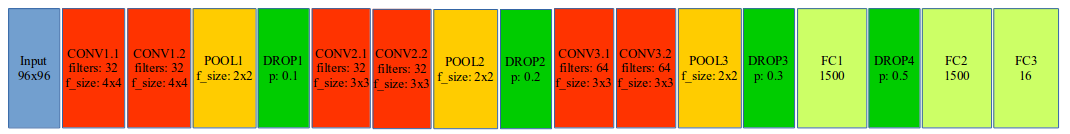
\includegraphics[scale=0.45]{images/ear_cnn2}
	\caption{The best architecture for automatic ear's landmarks detection}
	\label{1Econv}
\end{figure}
\subsubsection{Parameters}
The network was trained with $5000$ \texttt{epochs} and \texttt{batch size} of $128$. For each epoch, the dataset is randomly split into the training set and validation set. The number of images in the sets is divided with the ratio of $80\%:20\%$, respectively. The \texttt{learning rate} is set to $0.03$; and the initial of \texttt{momentum} is $0.9$. During training, the learning rate and momentum are re-calculated to adjust with the number of remaining epochs. All the parameters in model 1 are shown in Table \ref{celiaparameters}:
\begin{table}[h!]
	\centering
	\begin{tabular}{l l l}
	Parameter & Initial value & End value \\ \hline
	Epochs & 5000 &  \\ \hline
	Training batch size & 128 & \\ \hline
	Testing batch size & 128 & \\ \hline
	Learning rate & 0.03 & 0.00001 \\ \hline
	Momentum & 0.9 & 0.9999 \\ \hline
	\end{tabular}
	\caption{The network parameters in the Celia model}
	\label{celiaparameters}
\end{table}
\subsection{Model 2: Automatic beetle landmarks detection}
\subsubsection{Architecture}
From the tutorial of Daniel Nouri\footnote{http://danielnouri.org/} about using CNN to detect facial key points. We propose a CNN to detect the landmarks on pronotum. The proposed network includes three convolutional layers followed by three maximum pooling layers and three full connected layers(Fig.\ref{pmodel}). The network receives the gray-scale image ($256 \times 192$) as the input. The deep of convolutional layers is increased from $32, 64, $ to $ 128$ with different size of filter. The size of filters in pooling layers are kept in the same size of $2 \times 2$. At the end of network, three full-connected layers with the size of $500, 500, $ and $16$ are set up to predict the positions of landmarks. Besides, the model is designed with a small sharing learning-rate and the momentum. The learning-rate and the momentum are changed overtime of training.
\begin{figure}[h!]
	\centering
	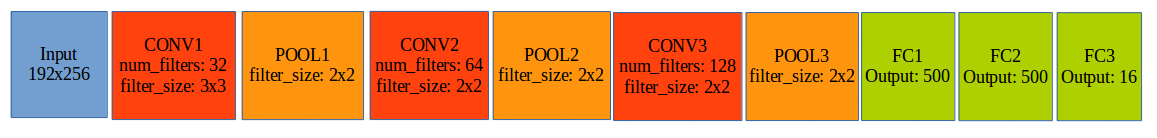
\includegraphics[scale=0.45]{images/model3}
	\caption{The architecture of proposed model}
	\label{pmodel}
\end{figure}
\subsubsection{Parameters}
The parameters in model 2 are shown in the Table \ref{model2parameters}:
\begin{table}[h!]
	\centering
	\begin{tabular}{l l l}
	Parameter & Initial value & End value \\ \hline
	Epochs & 5000 &  \\ \hline
	Training batch size & 128 & \\ \hline
	Testing batch size & 128 & \\ \hline
	Learning rate & 0.03 & 0.0001 \\ \hline
	Momentum & 0.9 & 0.9999 \\ \hline
	\end{tabular}
	\caption{The network parameters in proposed model}
	\label{model2parameters}
\end{table}
\section{Data}
\label{sectionData}
The experiment data includes 293 color images of pronotum. The images are divided into 3 subsets: training($200$ images), validation($60$ images) and testing set($33$ images). In which, the training and validation are combined to use as the input data of the networks(total $260$ images) during training. The images in testing set are used to evaluate the model. The images are chosen randomly to put into each set (after we have done some experiments).

Because the number of the images are limited (just $260$ color images), it does not enough to use for training process. Additional, the models are worked on gray-scale images. So, we applied some rules to enlarge the dataset. The first rule is adding a constant value to a channel of RGB image, we will have a new RGB image. For example, from an original $RGB$ image, if we add $10$ to red channel, we will have a new image $(R+10)GB$. Then, we apply the same rule with blue and green channel, we will obtain two new images: $R(G+10)B$ and $RG(B+10)$. By that way, from an RGB image, we can generate three RGB images by adding a constant to each channel(each time just change to a channel). The second rule is splitting the channels of RGB image (because the models work on gray-scale). It means that we can generate six versions from an original image. At the end, the number of the image in the training data is $ 260 \times 7 = 1820$ images (six versions and original). Before giving to the models, the images are down-sampled with the size of $256 \times 192$. The number of the images in training set and validation set are splitted automatically by the model's parameter.
\section{Experiments}
In practical, convergence is usually faster if the average of each input variable over the training set is close to zero. Because the values of the pixels and the coordinates of the landmarks are positive. If we consider that we stay at the a layer of the network, and the weights are updated by an amount proportional to $\delta x$($\delta$ is the scalar error at the layer and $x$ is the input vector). When the input vectors are positive, the updates of weights that feed into the layer will be the same sign($sign(\delta)$), it means that the weights can only all decrease or all increase together for a given input. That, if the weight vector change direction, it can only do by zigzagging which is inefficient and thus slow down learning. Therefore, it is good to shift the inputs so that the average over the training set is close to zero. Moreover, when the input is set closed with zero, it will more suitable with the sigmoid activation function\cite{lecun2012efficient}.
 
In this section, we describe the experimental processes of two models on pronotum dataset (section \ref{sectionData}). The experiments were conducted in the way pre-processing data before giving to the network. At the first experiment, the values of the images are normalized and the coordinates of the landmarks are kept as original. In the second experiment, both inputs are normalized before giving to the network. Then, some improvements are added into model 2 to obtain the better result.
\subsection{Experiment 1}
In the first experiment, the images are kept in gray-scale with the size of $256 \times 192$. The brightness of the image is normalized to $[0,1]$, instead of $[0,255]$ while the coordinates of the landmarks are kept as original. 
\subsubsection{With model 1}
We kept the same initial parameters of the model to train with the pronotum dataset. During training, the network cannot detect the loss of train and validation ($nan$ value). A solution is given that we decreased the initial value (from $0.03$ to $0.000001$) and the stop value (from $0.0001$ to $0.0000001$) of learning rate. The network is re-trained with new parameters and we have succeeded. Fig.\ref{model1loss} shows the losses during training and validation process. We can see that the losses are not stable between training and validation. Fig.\ref{model1test} shows the prediction landmarks on an image in test set (the network never saw before). The predicted landmarks are closed with the pronotum but their location is still inaccurate.
\begin{figure}[h!]
\centering
\subfloat[Training losses and validation loss]{\label{model1loss}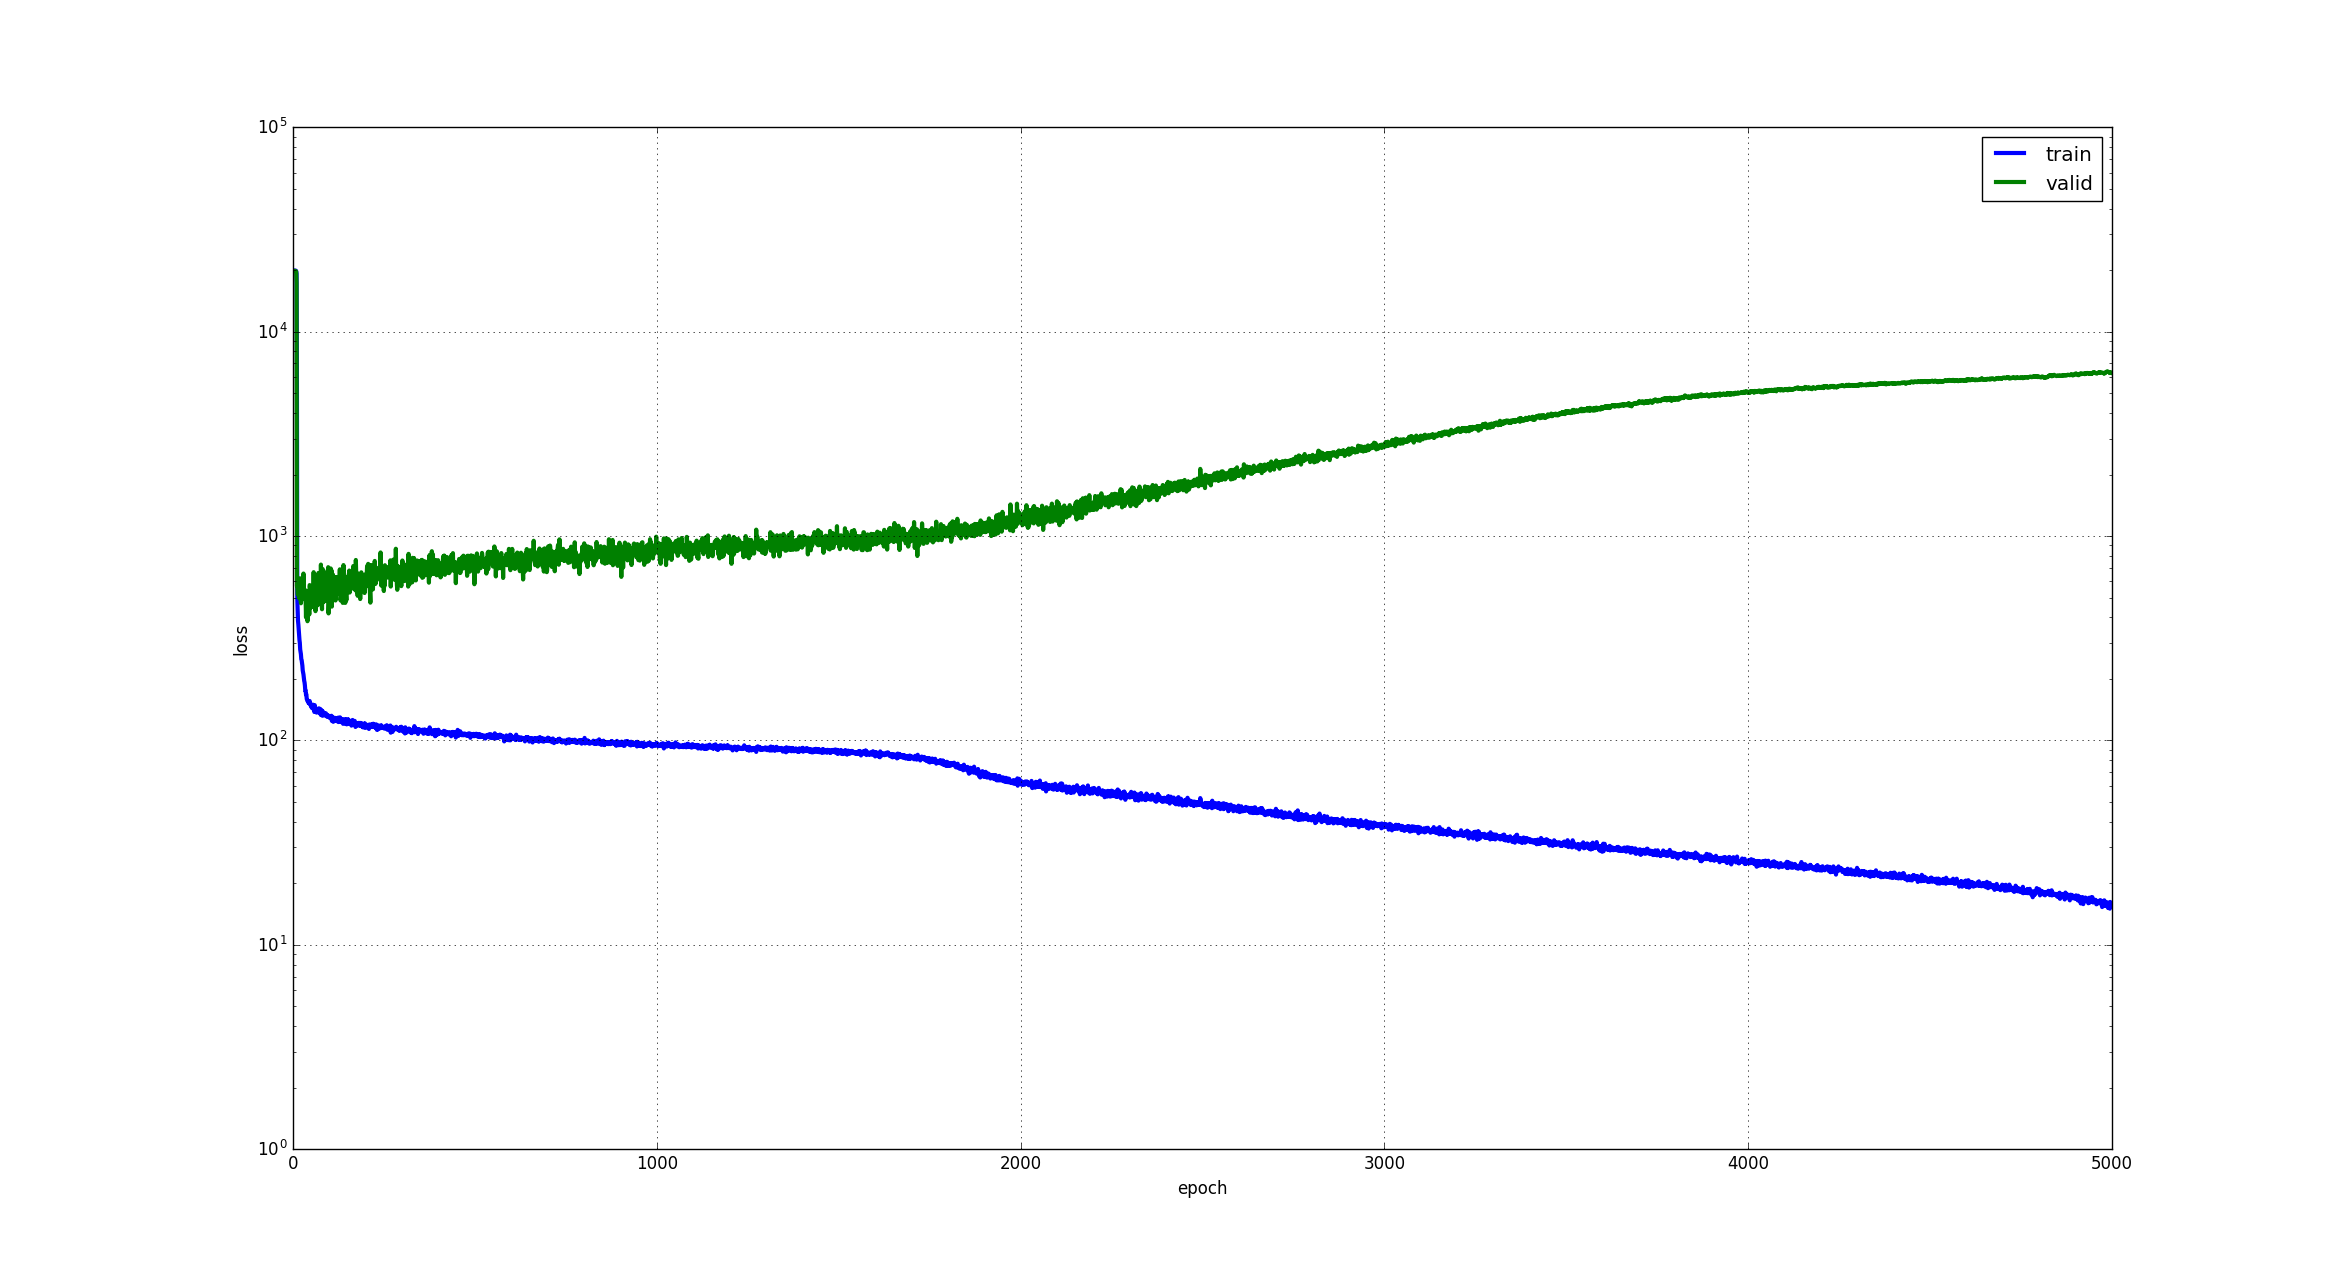
\includegraphics[width=0.5\textwidth]{./images/figure_1_celia_5000_without_normalize_data_loss}}~~
\subfloat[A pronotum with predicted landmarks]{\label{model1test}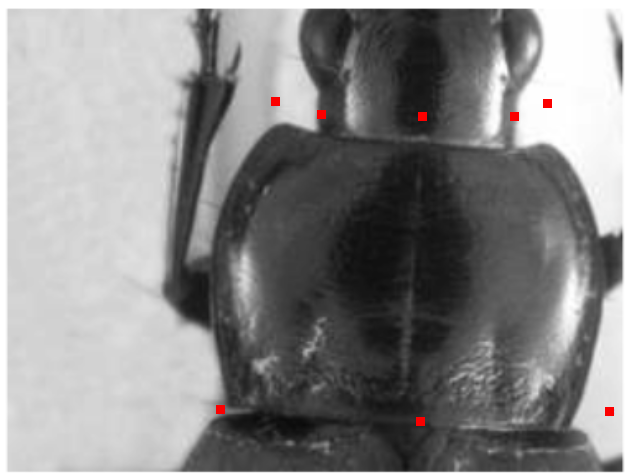
\includegraphics[width=0.5\textwidth]{./images/fig1_celia}}
\caption{The evaluation of pronotum data on model 1}
\label{model1tl}
\end{figure}
\subsubsection{With model 2}
From the experiment of model 1 on pronotum data. We change the learning rate in the model 2 before training the network: initial value is changed from $0.3$ to $0.00001$ and stop value is changed from $0.0001$ to $0.000001$. The training loss and validation loss are shown in Fig.\ref{model2loss}. The loss is stable to $1600$ epochs but then, they decreased to the end: $0.16694$ for training loss and $0.55584$ for validation loss. Clearly, when we compare the losses from two models, a difference has appeared, and the results of model 2 are worth considering. Fig.\ref{model2test} shown the predicted landmarks on a test image.
\begin{figure}[h!]
\centering
\subfloat[Training losses and validation loss]{\label{model2loss}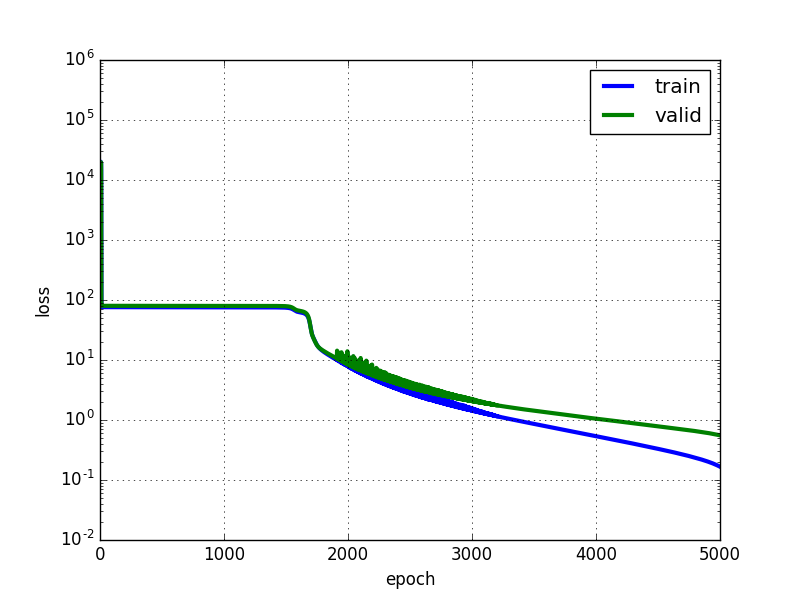
\includegraphics[width=0.5\textwidth]{./images/figure_1_cnn3_5000_loss_v13}}~~
\subfloat[A pronotum with predicted landmarks]{\label{model2test}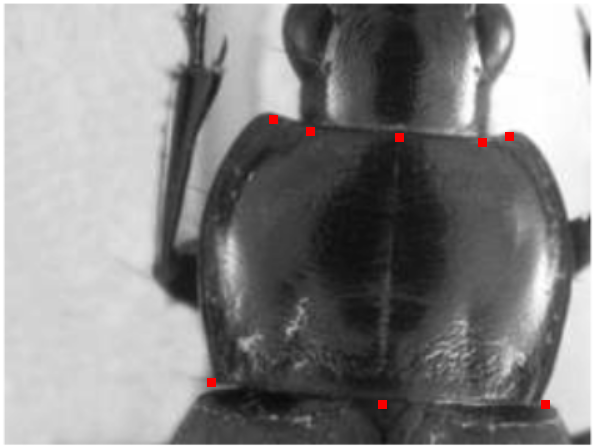
\includegraphics[width=0.5\textwidth]{./images/fig1_model2}}
\caption{The evaluation of pronotum data on model 2}
\label{model2tl}
\end{figure}
The model 2 is used to predict the landmarks on the test set (includes 33 images). Then, the correlation coefficient between manual and predicted landmarks is computed by using different correlation methods\cite{pallant2013spss,myers2010research,kendall1938new}. The correlation results are shown in Table.\ref{corr1}
\begin{table}[h!]
	\centering
	\begin{tabular}{l c c}
		Method & x correlation & y correlation \\ \hline
		Pearson & $0.9966784$ & $0.9957729$ \\ \hline
		Spearman & $0.9913126$ & $0.9565425$ \\ \hline
		Kendall & $0.9273012$ & $0.8273057$ \\ \hline
	\end{tabular}
	\caption{The correlation between manual and predicted landmarks on test images}
	\label{corr1}
\end{table}~\\[0.5cm]
\subsection{Experiment 2}
In the second experiment, both the image values and the target (landmark coordinates) are normalized to a range of $[-1,1]$, instead of $[0,256]$ and $[0,192]$ before giving to the networks\cite{lecun2012efficient}. After some trials, the learning rates are set at the beginning to increase the speed of the processes. Fig.\ref{expr2} show the loss during training and validation of two models with the new version of data. We can see that the losses from model 2 is really better than from model 1. But, at the end of training, the overfitting has appeared in model 2.
\begin{figure}[h!]
\centering
\subfloat[Model 1]{\label{model1loss2}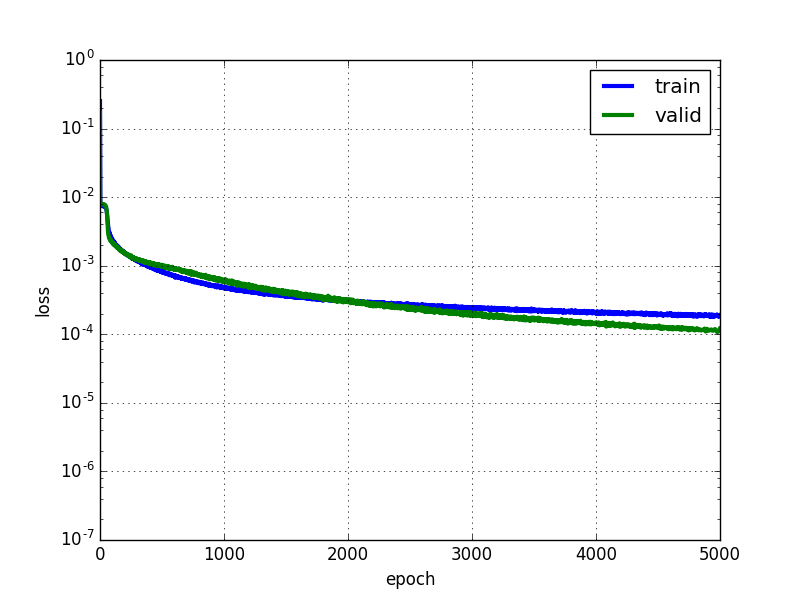
\includegraphics[width=0.4\textwidth]{./images/figure_1_loss_celia_5000_normalized_data}}~~
\subfloat[Model 2]{\label{model2loss2}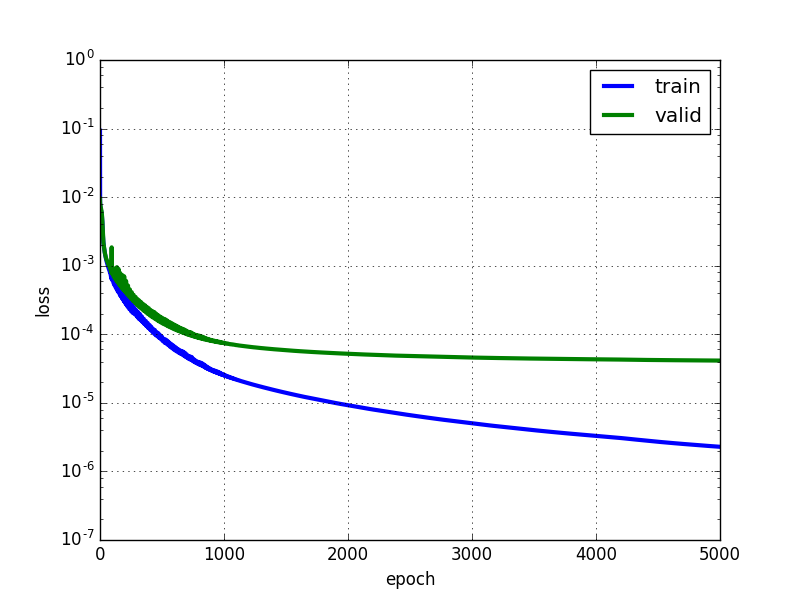
\includegraphics[width=0.4\textwidth]{./images/cnnmodel3_5000_pronotum_v13_without_dropout_normalized_data_loss}}
\caption{The training and validation loss on two models}
\label{expr2}
\end{figure}~\\
To prevent the overfitting on the model 2, we have changed the ratio of train/val selection. The new ratio is set to $60\%:40\%$, instead of $80\%:20\%$ as the beginning. The network is re-train with the new data but the overfitting is also not stopped. Then, we decide to modify the structure of the network (Fig.\ref{model2dropout}):
\begin{itemize}
	\item Increasing the number of output at the last two hidden layers (full-connected) from $500$ to $1000$, but the result did not lead to better performances,
	\item Then, we added four dropout layers to the network. The dropout layer is considered as the good solution to prevent the overfitting\cite{srivastava2014dropout}. They have been located following the pooling layers and the first fill-connected layer. The dropout ratios are $0.1$, $0.2$, $0.3$ and $0.5$.
\end{itemize}
\begin{figure}[h!]
	\centering
	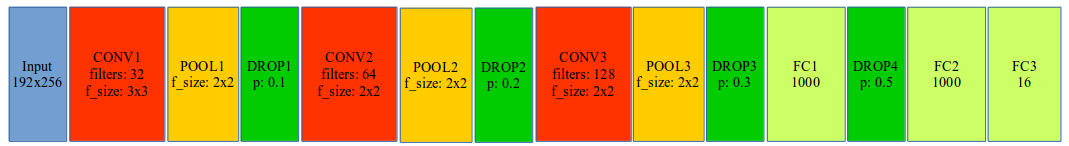
\includegraphics[scale=0.35]{images/model3_dropout}
	\caption{The proposed model with dropout layers}
	\label{model2dropout}
\end{figure}~\\
Fig.\ref{tvldropout} shows the losses after the model have been modified. The overfitting problem has been solved but the losses are stability from $2000^{th}$ until the end(we need more data). 
\begin{figure}[h!]
	\centering
	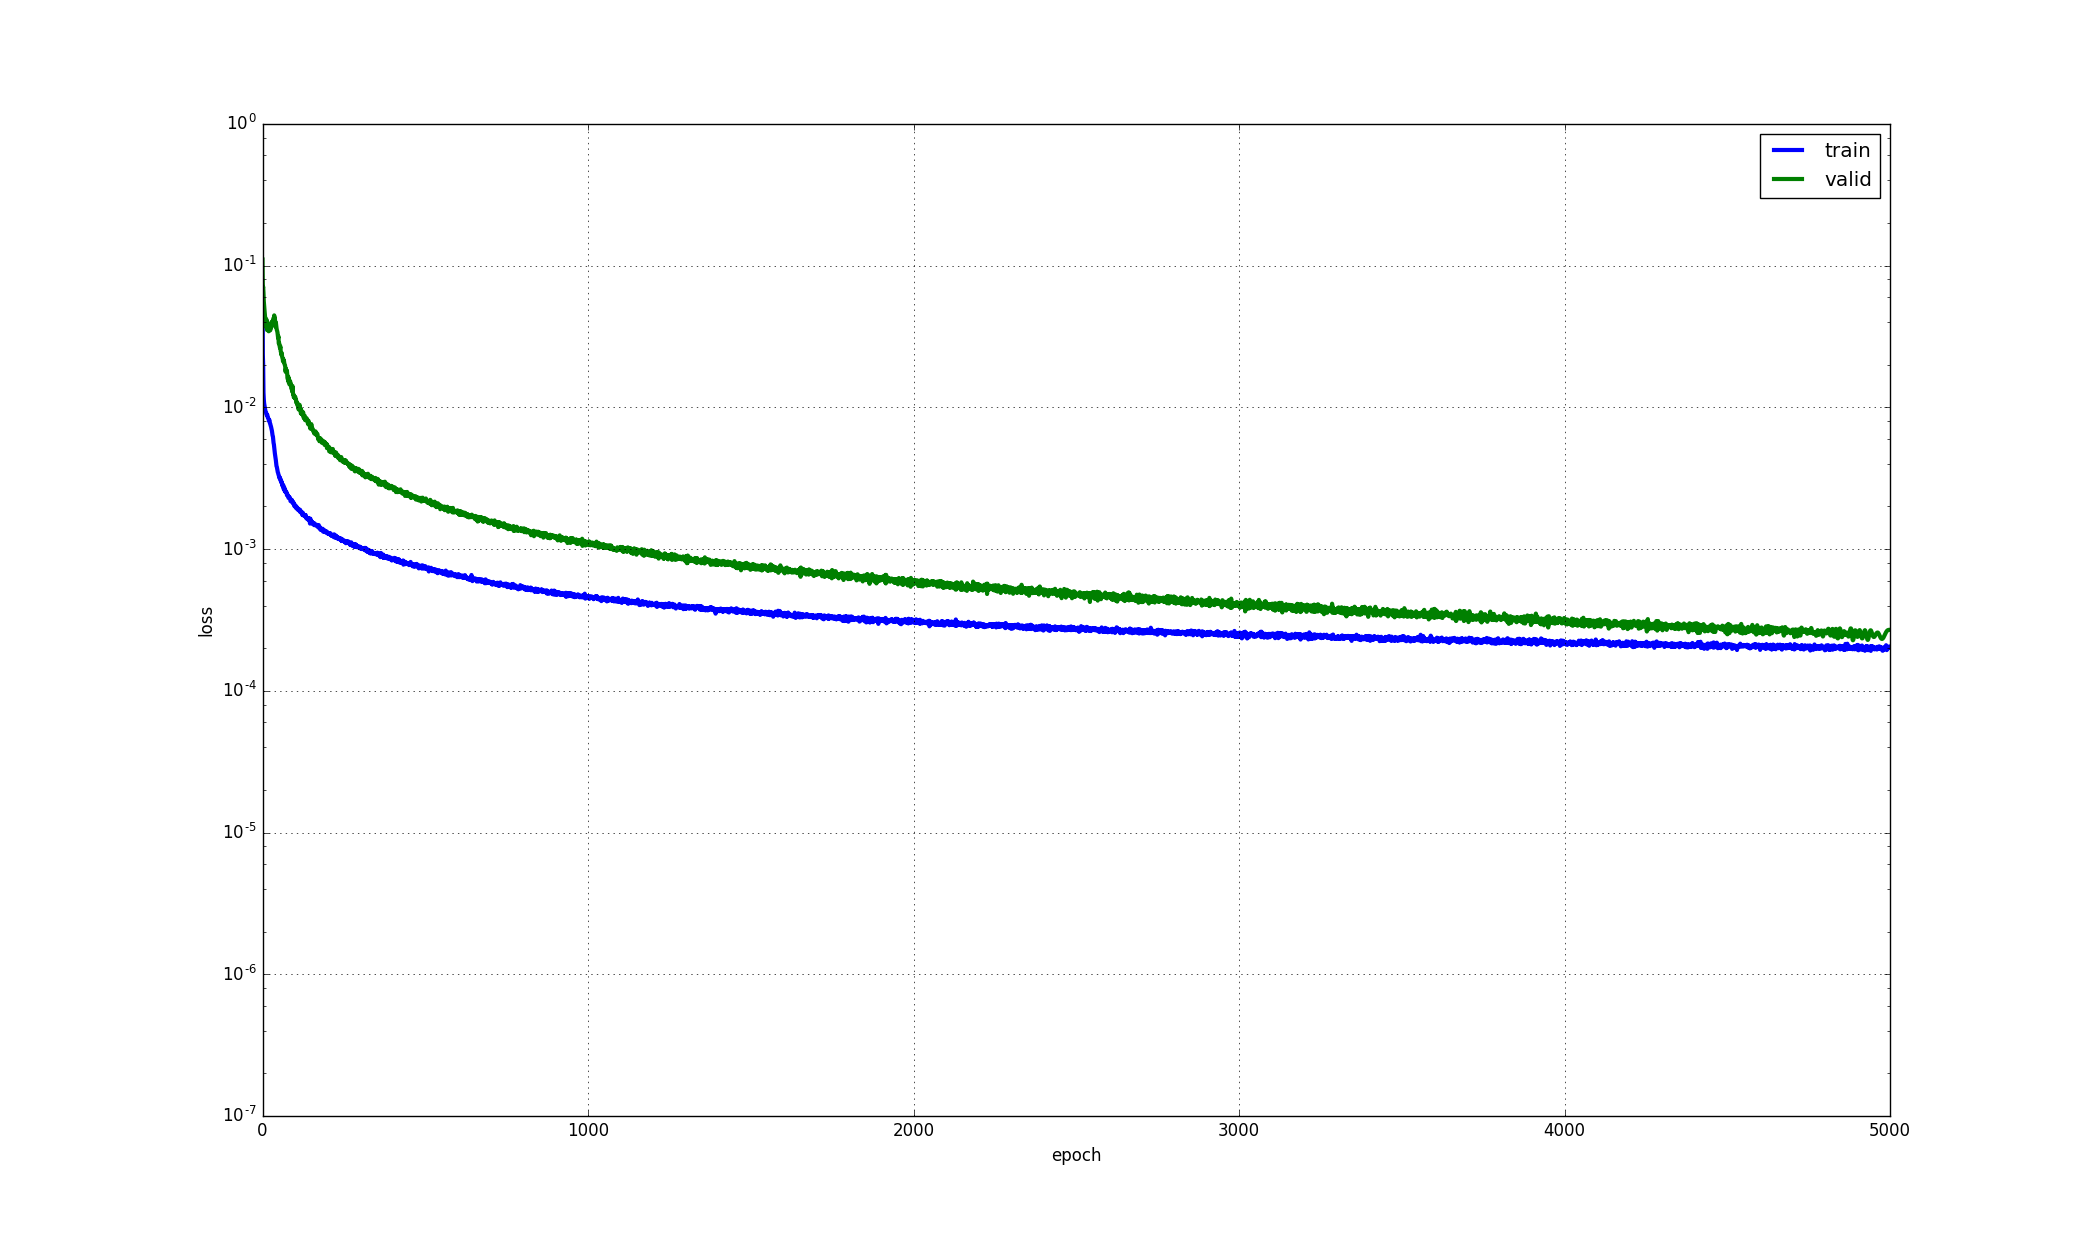
\includegraphics[scale=0.17]{images/figure_1_cnn3_3000_v13_loss_change3_dropout_increase_2}
	\caption{The training and validation loss with dropout layers}
	\label{tvldropout}
\end{figure}~\\
Fig.\ref{expr22} and show the predicted landmarks on an image in test dataset. 
\begin{figure}[h!]
\centering
\subfloat[Model 1]{\label{model1loss2}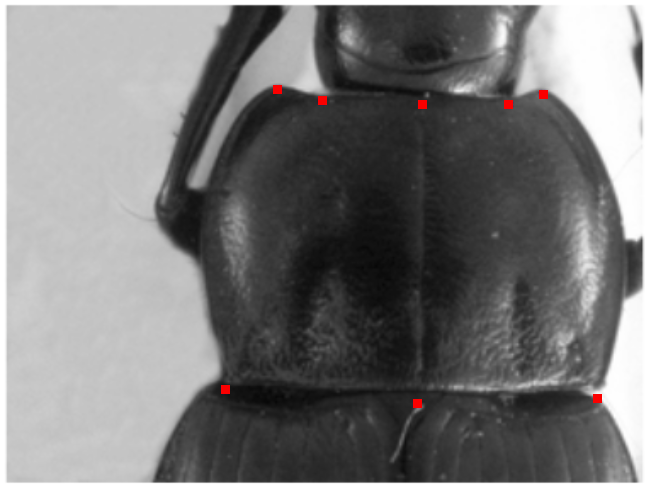
\includegraphics[width=0.4\textwidth]{./images/fig2_celia}}~~
\subfloat[Model 2]{\label{model2loss2}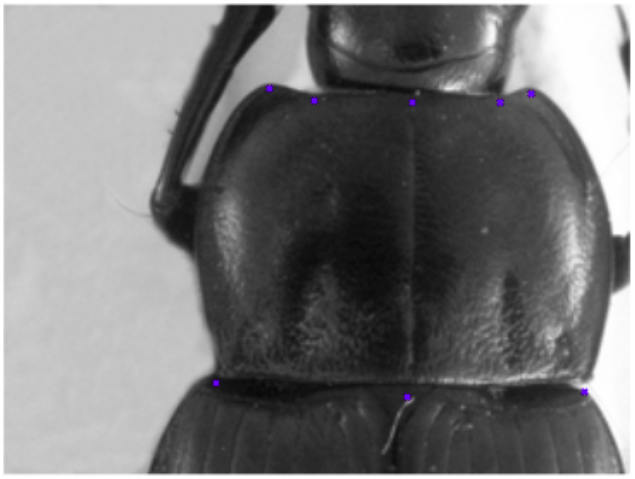
\includegraphics[width=0.4\textwidth]{./images/fig2_model2}}
\caption{The predicted landmarks on a test image}
\label{expr22}
\end{figure}~\\
Both models are evaluated on test set. Table \ref{coffcelia} shows the correlation coefficient of model 1 and Table \ref{coffdropout} shows the correlation coefficient of model 2. Clearly that, the result from model 2 have been improved a little bit when we compare with the last result(Table \ref{corr1}). While we do not see the difference between the results of model 1 and model 2. The only difference is the architecture of the models: model 1 is deeper than model 2 that means the model 1 takes more time to train than the model 2.
\begin{table}[h!]
	\centering
	\begin{tabular}{l c c}
		Method & x correlation & y correlation \\ \hline
		Pearson & $0.9976008$ & $0.9983418$ \\ \hline
		Spearman & $0.9948408$ & $0.9875125$ \\ \hline
		Kendall & $0.9463506$ & $0.9133915$ \\ \hline
	\end{tabular}
	\caption{The correlation between manual and predicted landmarks on pronotum images with model 1}
	\label{coffcelia}
\end{table}
\begin{table}[h!]
	\centering
	\begin{tabular}{l c c}
		Method & x correlation & y correlation \\ \hline
		Pearson & $0.9970585$ & $0.9978605$ \\ \hline
		Spearman & $0.9942475$ & $0.9859642$ \\ \hline
		Kendall & $0.9430501$ & $0.9067739$ \\ \hline
	\end{tabular}
	\caption{The correlation between manual and predicted landmarks on pronotum images with model 2}
	\label{coffdropout}
\end{table}~\\
Besides the evaluation on correlation coefficient, we also consider the accuracy on each landmark of all images in the test set. The distance between manual landmark and predicted landmark is calculated. Then, the standard deviation(SD) is used to quantify the dispersion of a set of distances. Fig.\ref{expr22s} show the statistic on each landmark of test dataset(from two models). All landmarks have been detected with an accuracy greater than $70\%$ (excepts $3^{rd}$ landmark).  The first model provided the good accuracy for $2^{nd}, 5^{th}, 8^{th}$ landmarks, while the second model had the good position for $4^{th}, 5^{th}, 6^{th}$ landmarks. Generally, we can see a vast difference between the correlation coefficient result and the proportion on each landmark.
\begin{figure}[h!]
\centering
\subfloat[Model 1]{\label{model1loss2}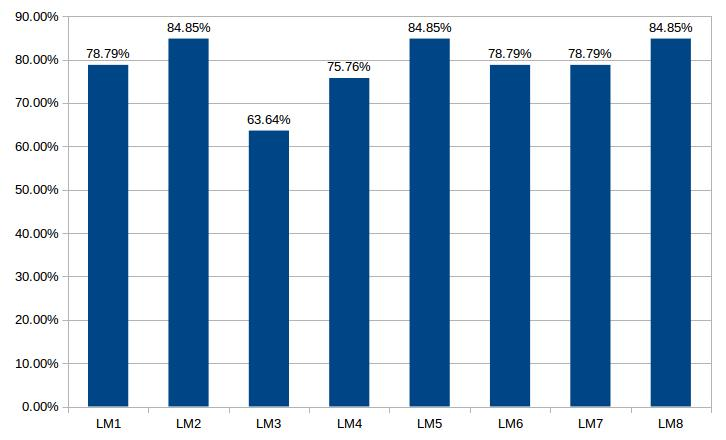
\includegraphics[width=0.5\textwidth]{./images/pronotum_celia_statistic}}~~
\subfloat[Model 2]{\label{model2loss2}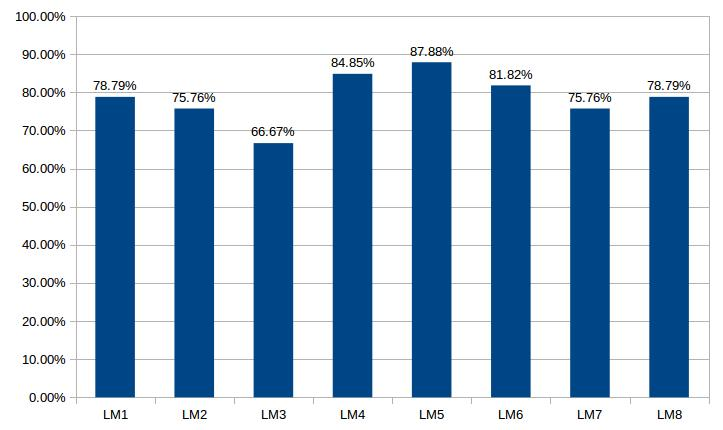
\includegraphics[width=0.5\textwidth]{./images/pronotum_pmodel_statistic}}
\caption{The proportions of well predicted landmarks on each model}
\label{expr22s}
\end{figure}~\\
The average distances and standard deviations of all landmarks are shown in Table \ref{sdmodel1} and Table \ref{sdmodel2}.
\begin{table}[h!]
	\centering
	\begin{tabular}{l c c c c c c c c}
		Landmarks & LM1 & LM2 & LM3 & LM4 & LM5 & LM6 & LM7 & LM8 \\ \hline
		Average & 3.6758 &	3.8836 & 	2.9337 & 	4.4401 &	 3.8504 &	4.5767 &	 3.0965 &	4.5527

 \\ \hline
		SD & 2.5006 &	3.0874 & 	1.6591 & 	3.0579 & 	3.1195 &	 3.9012 &	2.4359 &	3.8919
 \\ \hline
	\end{tabular}
	\caption{The average distance and standard deviations from model 1}
	\label{sdmodel1}
\end{table}~\\
\begin{table}[h!]
	\centering
	\begin{tabular}{l c c c c c c c c}
		Landmarks & LM1 & LM2 & LM3 & LM4 & LM5 & LM6 & LM7 & LM8 \\ \hline
		Average & 4.2249 & 4.7678 & 3.6129 &	4.4391	 & 4.4319	& 5.2091 &	 4.1567 &	5.1568
 \\ \hline
		SD & 2.6985 &	3.06024 & 1.6963	& 3.6506 & 	3.4997 &	4.2616 &	2.5724 &	3.8691
 \\ \hline
	\end{tabular}
	\caption{The average distance and standard deviations from model 2}
	\label{sdmodel2}
\end{table}~\\
\section{Conclusions}
Two models that used to predict the landmarks on 2D gray-scale images are studied. For each case, the model is suitable with different dataset but the results are still good when we change the training data (the case of model 1 when we re-train on pronotum). Besides, we proposed a different way to enlarge the data in the case the dataset is limited. From the correlation coefficients of each model shows that the effects of two models are similar. Additional, if we consider on the statistic side, the coefficients are enough good to precise. But, when we see the predicted landmarks on the images, we also have some case that is not good as we expect. 
\bibliographystyle{unsrt}
\bibliography{includes/references}
\pagebreak
\appendix
\section*{A comparison on parameters of the networks}
The number of layers in each model are shown in Table \ref{numlayers}.
\begin{table}[h!]
	\centering
	\begin{tabular}{l p{1.2cm} p{3cm} p{2cm} p{1.2cm} p{2cm} p{2cm}}
		Model & $N^o$ layers & Input size & $N^o$ CONVs & $N^o$ POOLs & $N^o$ Dropout & $N^o$ FC \\ \hline
		model 1 & 16 & $1 \times 96 \times 96$ & 6 & 3 & 4 & 3 \\ \hline
		model 2 & 9 & $1 \times 256 \times 192$ & 3 & 3 & 0 & 3 \\ \hline
		model 2\_1 & 9 & $1 \times 256 \times 192$ & 3 & 3 & 0 & 3 \\ \hline
		model 2\_2 & 13 & $1 \times 256 \times 192$ & 6 & 3 & 4 & 3 \\ \hline
	\end{tabular}
	\caption{The number of layer types in each model}
	\label{numlayers}
\end{table}~\\
The detail parameters in each layer of the models are shown in Table \ref{modelparameters}.
\begin{table}[h!]
	\centering
	\begin{tabular}{l p{3cm} p{3cm} p{3cm} p{3cm}}
		layers & model 1 & model 2 & model 2\_1 & model 2\_2 \\ \hline
		input & $ 1 \times 96 \times 96$ & $1 \times 256 \times 192$ & $1 \times 256 \times 192$ & $1 \times 256 \times 192$ \\ \hline
 		layer 1 & CONV(32,4,1,0) & CONV(32,3,1,0) & CONV(32,3,1,0) & CONV(32,3,1,0) \\ \hline
		layer 2 & CONV(32,4,1,0) & POOL(2,2,0) & POOL(2,2,0) & POOL(2,2,0) \\ \hline
		layer 3 & POOL(2,2,0) & CONV(64,2,1,0) & CONV(64,2,1,0) & \textbf{DROP(0.1)} \\ \hline
		layer 4 & DROP(0.1) & POOL(2,2,0) & POOL(2,2,0) & CONV(64,2,1,0) \\ \hline
		layer 5 & CONV(32,3,1,0) & CONV(128,2,1,0) & CONV(128,2,1,0) & POOL(2,2,0) \\ \hline
		layer 6 & CONV(32,3,1,0) & POOL(2,2,0) & POOL(2,2,0) & \textbf{DROP(0.2)} \\ \hline
		layer 7 & POOL(2,2,0)  & FC(500) & FC(\textbf{1000}) & CONV(128,2,1,0) \\ \hline
		layer 8 & DROP(0.2) & FC(500) & FC(\textbf{1000}) & POOL(2,2,0) \\ \hline
		layer 9 & CONV(64,3,1,0)  & FC(16) & FC(16) & \textbf{DROP(0.3)} \\ \hline
		layer 10 & CONV(64,3,1,0)  & - & - & FC(1000) \\ \hline
		layer 11 & POOL(2,2,0) & - & - & \textbf{DROP(0.5)} \\ \hline
		layer 12 & DROP(0.3) & - & - & FC(1000) \\ \hline
		layer 13 & FC(1500) & - & - & FC(16) \\ \hline
		layer 14 & DROP(0.5) & - & - & - \\ \hline
		layer 15 & FC(1500) & - & - & - \\ \hline
		layer 16 & FC(16) & - & - & - \\ \hline
	\end{tabular}
	\caption{The parameters at each layer of the models}
	\label{modelparameters}
\end{table}~\\
Which:
\begin{itemize}
	\item CONV(x,y,z,t): convolutional layer with the parameters: \textit{x = number of filters, y = size of filter matrix, z = stride value, t = padding value}
	\item POOL(y,z,t): maximum pooling layer with: \textit{y = size of filter, z = stride value, t = padding value}
	\item DROP(p): dropout layer with \textit{p is the dropout ratio}
	\item FC(x): full-connected layer with \textit{x is the number of output}
\end{itemize}

\end{document}